\setlength{\parindent}{0ex}
\setlength{\parskip}{2ex}

\chapter{Conclusion}

In my thesis I have investigated the selective forces that shape genetic variation within populations and between species. In Chapter 2, I showed that positive selection contributes significantly to divergence in coding and noncoding regions, reduces linked neutral diversity, and that variation in gene expression influences the strength of selection on genes. In Chapter 3, I mapped the loci that affect local control of gene expression and demonstrated that negative selection is the strongest force acting on these loci, consistent with mutation-selection balance. In Chapter 4, I investigated the role of pleiotropy in shaping how selection acts on genes, showing that genes with more and stronger network connections experience stronger negative and positive selection. Throughout my thesis I have used gene expression as a tool to link genotype to phenotype in an effort to develop a holistic view about how selection shapes genetic variation at the genetic and phenotypic level. In this chapter I describe the implications of my results.

\section{What forces maintain genetic variation?}

On the genome-wide scale, mutation-selection balance appears to be pervasive. I saw this at both the sequence level, where it appears that the dominant force acting on within-population genetic variation is negative selection, and at the phenotypic level, where eQTLs appear to be under negative selection. One caveat to this conclusion is that, at the phenotypic level, we were only able to detect eQTLs at relatively high allele frequencies, suggesting that most of the variation we did observe was at most only weakly deleterious.

While I was able to describe the selective forces acting on eQTLs in my thesis, I was unable to explain how much of additive genetic variation ($V_{a}$) for expression is explained by these eQTLs, and ultimately, by mutation-selection balance (as in \citealt{monnahan2015}). The selective forces maintaining genetic variation for a trait may differ from the forces that maintain variation for the QTLs that determine trait value in some cases. For example, if a trait\textsc{\char13}s value is determined by genotype at 99 rare small-effect QTLs and 1 common large effect QTL, we might conclude that the QTLs for the trait are under mutation-selection balance while most of the $V_{a}$ observed for the trait is neutral or under balancing selection. This scenario seems unlikely in my experiments because we have more power to detect the large-effect common QTLs that also will contribute more to $V_{a}$. However, it would be satisfying to find a way to directly estimate the impact of mutation-selection balance on expression variation.

My results do not mean that balancing selection is unimportant, just that it does not shape genetic variation on a genome-wide scale in a way that would be detectable with the approaches that I used. There is already one example of a polymorphism involved in speciation that is maintained by balancing selection within \textit{C. grandiflora} \citep{Sicard2015-uc}. One future direction could be to search for isolated instances of balancing selection acting on genic sequence or maintaining polymorphism in eQTLs. This analysis will be difficult because we lack clear theoretical predictions for the selective signatures that will be left by balancing selection, but finding signatures of long, intermediate-frequency haplotypes surrounding intermediate-frequency large-effect eQTLs would be consistent with the action of balancing selection.

\section{Linking population genetics and quantitative genetics}

Throughout my thesis I have interacted with two different ways of viewing evolution: population genetics and quantitative genetics. To put these two fields in context, it might be helpful to refer to \citet{lewontin1974}, who described how a population moves from genotype space to phenotype space, where selection occurs, and back to genotype space, which preserves information for the next generation.


\begin{figure}[ht!]
      \centering
       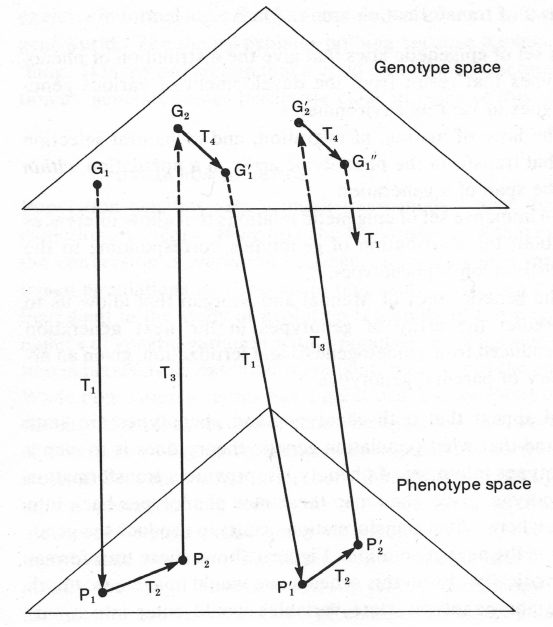
\includegraphics[scale=0.8]{figure_no_caption}
    \caption{\textbf{Schematic representation of the paths of transformation of population genotype from one generation to the next.} Taken from \citet{lewontin1974}.}
    \label{fig:lew}
\end{figure}

The field of population genetics tracks populations on the genotype plane, collapsing information about phenotype and selection into the parameters $s$, the strength of selection, . Using population genetic techniques, I can estimate the $s$ acting on a specific sequence, which is incredibly powerful. In contrast, quantitative genetics focuses on movement in the phenotype, or “form”, plane, collapsing details about the genetic basis of these responses into $V_{a}$, $V_{g}$, and $h^{2}$, which are themselves notoriously unintuitive parameters. These differing perspectives can lead to different ideas about how selection works. For example, the population genetics view that each genetic variant has a defined, constant, $s$ conflicts with the quantitative genetics view of selection acting on the composite value of allelic effects at all loci.

\citet{lewontin1974} argued that evolutionary biology needs a unified theory that combines the population and quantitative genetics views to fully describe evolutionary processes. However, this has proved challenging. While quantitative genetics and population genetics make up two sides of Lewontin\textsc{\char13}s diagram, their differing origins and perspectives can be hard to reconcile. During my thesis I have mainly sought to combine the insights from both of these fields by using phenotypic information to construct categories of genes or loci based on their phenotypic associations and then use population genetics to describe the selective forces acting on these categories. There have been many limitations to this approach and it is a far cry from truly uniting these two fields. Now that genomics allows us to both see the infinitesimally small mutations described by quantitative genetics and to link traits of interest to the genetic loci described by population genetics, it seems promising that we will be soon able to develop a fully combined evolutionary genetics theory.

